%\chapter{Model-View-Controller}\fxfatal{Der er ingen kilder på dette afsnit? og linjebrud i kildefilen er volsomt træls. - Troels}\fxfatal{Tror hele dette afsnite skal omskrives til at følge: ``A model represents the state of a particular aspect of the application. A controller handles interactions and updates the model to reflect a change in state of the application, and then passes information to the view. A view accepts necessary information from the controller and renders a user interface to display that information.'' Fra wikipedia: \url{http://en.wikipedia.org/wiki/ASP.NET_MVC_Framework}}
%Model-View-Controller(MVC) er et designmønster som fordeler 
%objekter\fxnote{Det fordeler logik over 3 lag ... ikke objekter. - Troels} i en applikation ud på tre forskellige roller, 
%Model, View og Controller. Hver enkelt rolle er separeret fra 
%hinanden, hvilket gør koden lettere at håndtere, teste og strukturere.

%\textbf{Model} laget er skjult for brugeren. Dette lag bør 
%indeholde det mest grundlæggende data for applikationen, 
%dette værende diverse klasser der benyttes, data der bruges 
%gentagende gange i applikationen. Denne data kan være gemt i en database eller i lokale filer, og bør indlæses som objekter. Model 
%objekter skal repræsenterer viden og erfaring inden for et 
%givent problemområde, hvilket også tillader et godt adskilt 
%modellag, at blive genbrugt i andre lignende områder. På 
%samme tid er det i dette lag hvor validerings logik, og andre 
%data beregninger på objekter skal udføres. Om muligt skal 
%et objekt i model laget ikke have nogen forbindelse til 
%View laget, således der ikke er nogen direkte forbindelse til 
%brugergrænsefladen. Kommunikation mellem dette lag og hvad 
%brugeren ser, skal ske igennem Controller laget.\fxfatal{Hvis dette er sandt fatter jeg totalt meget hat af denne figur: \url{http://www.cs.cf.ac.uk/Dave/HCI/HCI_Handout_CALLER/MVC.gif} }
%
%\textbf{View} laget er hvad brugeren kan se. Et objekt i view 
%laget bruges primært til at fremvise data, samt tillade 
%brugere at ændre data i model laget. På trods af den 
%interaktion der er mellem lagene, er de frakoblet hinanden, 
%kommunikation om opdatering af data, samt ændringer brugeren 
%laver sker igennem Controller objekter. Essentielt er det en 
%visuel repræsentation af den data der ligger i model laget.
%
%\textbf{Controller}
%Controller objekter fungerer som mellemled mellem objekter i 
%model og view lagene. Derved bliver controller objekter til 
%et kommunikationsværktøj mellem model og view lag. En brugers 
%aktion på et objekt i view laget, fortæller et controller 
%objekt om bruger aktionen, hvorefter controller objektet 
%kontakter de objekter i model laget det vedrører, her 
%behandles informationen og bliver på samme måde sendt tilbage 
%til view laget og giver derved brugeren respons.

\chapter{MVC-mønsteret}
Et af de standardiserede design mønstre, som bruges af mange udviklere er MVC-mønsteret - som står for \textit{Model-View-Controller}.
MVC-mønsteret har til formål, at dele systemet op i tre komponenter, nemlig \textit{Model}, \textit{View} og \textit{Controller}.
Denne segregering adskiller således ''forretnings-logik'', ''input-logik'' og ''UI-logik'', og gør herved systemet mere fleksibelt, samt fremmer muligheden for at udvikle parallelt på de forskellige komponenter.
Dette kan være nyttigt i udviklingen af systemet, men også efter udgivelsen, idet blandt andet ''UI-logik''har det med at blive ændret oftere end for eksempel ''forretnings-logik''. 
Opdelingen hjælper også til at skabe overblik over koden, og gør det nemmere at udføre tests på systemet. \citep{MVC_Overview}

\begin{wrapfigure}{r}{0.4\textwidth}
	\vspace{-20pt}
	\begin{center}
		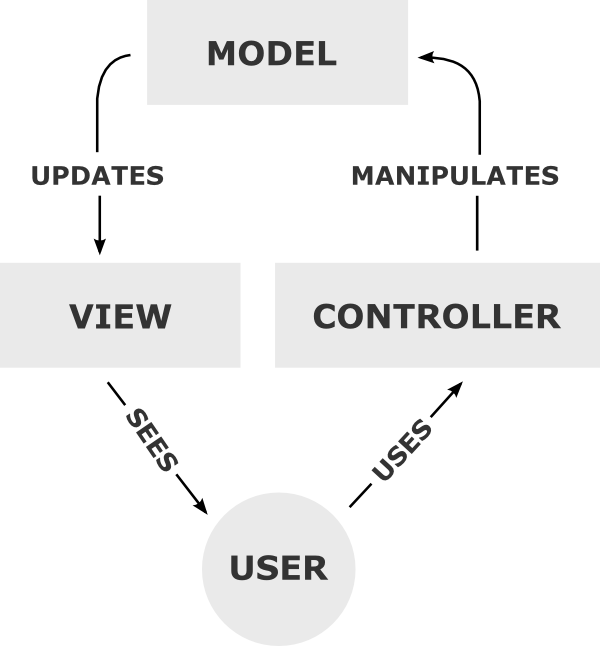
\includegraphics[width=0.38\textwidth]{images/Images/mvc.png}
	\end{center}
	\vspace{-20pt}
	\caption{MVC-mønsteret}
	\vspace{-20pt}
\end{wrapfigure}
	

Nedenfor beskriver vi de tre komponenter.

\textbf{Model}\\
De objekter, der udgør model-laget skal indeholde den før omtalte ''forretnings-logik'', samt alle data der skal modeleres i systemet.
Data'en, i form af objekter, gemmes oftest i en database eller fil, og er helt skjult for brugeren i den forstand, at al repræsentation af modellen foregår igennem view-delen af MVC-mønsteret. 

\textbf{View}\\
Der er igennem forskellige views, at brugeren får præsenteret brugergrænsefladen - også kaldet UI(user-interface).
Derfor giver det også mening, at placere ''UI-logikken'' i denne del af MVC-mønsteret.
Typisk bliver et views indhold genereret ud fra data fra en model.
Et eksempel på dette ville være visning af en liste af objekter ud fra en model, der indeholder netop en liste.

\textbf{Controller}\\
Når det kommer til interaktionen mellem brugeren og systemet, er det controlleren der påtager sig opgaven.
Derfor er det også i de forskellige controllerere, at vi finder ''input-logikken''. Her bestemmes udfra input fra brugeren hvilke data der skal arbejdes med i hvilken model og også hvilket view, der skal præsenteret for brugeren. Med dette kan vi også se, at viewet ikke indeholder noget logik og al manipulation af data altså foregår gennem controller komponenten.
